%%%
%
% $Autor: Shubhankar Dumka, Gautam Ramesh, Siddhanth Sharma $
% $Date: 2026-01-24 $
% $File: KDD2.tex $
% $Version: 1.0 $
%
% !TeX spellcheck = en_GB
% !TeX program = pdflatex
% !TeX encoding = utf8
%
%%%

% This file continues the KDD section introduced in KDD1.tex.

\usetikzlibrary{arrows.meta, positioning}

\chapter{Knowledge Discovery in Databases (KDD) - Data Transformation}
\label{ch:kdd_data_transformation}
\index{Knowledge Discovery in Databases (KDD) - Data Transformation}

\section{Data Transformation}
\label{subsec:kdd_data_transformation}
\index{Knowledge Discovery in Databases (KDD) - Data Transformation}

In the KDD process, \textit{data transformation} is the final conversion step that produces the \textbf{exact input representation required by the model}. In this project, earlier \textit{data processing} (cleaning, labeling checks, augmentation) is performed offline during dataset preparation, while \textit{data transformation} is performed \textbf{per frame} just before inference (and equivalently inside the training loader during training runs).

\begin{figure}[htbp]
	\centering
	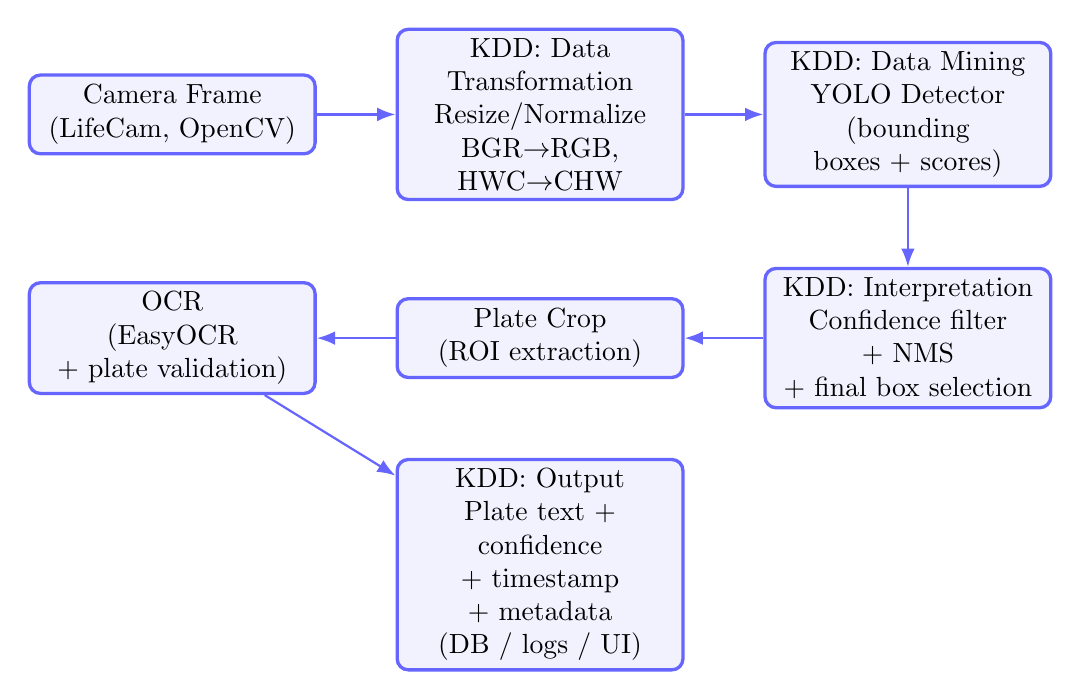
\begin{tikzpicture}[
	node distance=10mm and 10mm,
	box/.style={
		rectangle,
		draw=blue!60,
		fill=blue!5,
		very thick,
		rounded corners,
		align=center,
		text width=0.28\linewidth,
		minimum height=10mm
	},
	arrow/.style={-Latex, thick, blue!60}
]

	\node[box] (frame) {Camera Frame\\(LifeCam, OpenCV)};
	\node[box, right=of frame] (transform) {KDD: Data Transformation\\Resize/Normalize\\BGR$\rightarrow$RGB, HWC$\rightarrow$CHW};
	\node[box, right=of transform] (mining) {KDD: Data Mining\\YOLO Detector\\(bounding boxes + scores)};

	\node[box, below=of mining] (interpret) {KDD: Interpretation\\Confidence filter\\+ NMS\\+ final box selection};
	\node[box, left=of interpret] (crop) {Plate Crop\\(ROI extraction)};
	\node[box, left=of crop] (ocr) {OCR\\(EasyOCR\\+ plate validation)};

	\node[box, below=of crop] (output) {KDD: Output\\Plate text + confidence\\+ timestamp + metadata\\(DB / logs / UI)};

	\draw[arrow] (frame) -- (transform);
	\draw[arrow] (transform) -- (mining);
	\draw[arrow] (mining) -- (interpret);
	\draw[arrow] (interpret) -- (crop);
	\draw[arrow] (crop) -- (ocr);
	\draw[arrow] (ocr) -- (output);

\end{tikzpicture}

	\caption{Runtime KDD mapping of the license plate pipeline from camera frame to final output knowledge product.}
	\label{fig:kdd_runtime_pipeline}
\end{figure}

\paragraph{Concrete transformations applied before model execution}
For each camera frame, the following formatting transformations are applied immediately before the detector runs (tool-specific requirements that do not change the semantic meaning of the frame):
\begin{itemize}
	\item \textbf{Resize to model input size:} the camera frame is resized to \(640\times640\) pixels for the detector engine input.
	\item \textbf{Pixel normalization:} pixel values are converted from \texttt{uint8} in \([0,255]\) to \texttt{float32} in \([0.0,1.0]\).
	\item \textbf{Channel order:} OpenCV provides frames as BGR; the inference engine expects RGB (\texttt{BGR\(\rightarrow\)RGB}).
	\item \textbf{Tensor layout:} the input is converted from \(\text{H}\times\text{W}\times\text{C}\) to \(\text{C}\times\text{H}\times\text{W}\), then flattened to match the TensorRT input binding.
\end{itemize}

\paragraph{Where the transformation happens (Jetson vs.\ offline)}
In the deployed system, these transformations are executed \textbf{on the Jetson Nano in real time} for every frame coming from the LifeCam. During development/training, the same conventions are applied in the training pipeline so that the network sees inputs with the same scale and channel conventions as in deployment.

\paragraph{Why the transformations are required}
The deployed detector runs as a TensorRT engine, which requires a fixed input tensor shape and numeric format. Without resizing, normalization, and correct channel ordering/layout, the engine cannot be executed correctly and detection results become unstable or invalid.

\section{Data Mining}
\label{subsec:kdd_data_mining}

\subsection{Data Mining Application}
\label{subsec:kdd_hyperparameters}

For this application, the mined pattern is the \textbf{presence and location of a license plate} in an image.

\paragraph{Task type}
The data mining task is \textbf{supervised learning} in the form of \textbf{object detection}:
\begin{itemize}
	\item \textbf{Localization:} regress bounding boxes around license plates.
	\item \textbf{Classification:} assign the ``license plate'' class to each predicted box.
\end{itemize}

\paragraph{Technique and justification}
We use a \textbf{YOLO-based detector} because it provides a strong speed--accuracy trade-off for small objects (license plates) and is suitable for real-time inference on constrained edge hardware. The detector is trained/fine-tuned in a PyTorch workflow and then deployed as an \textbf{optimized TensorRT engine} on the Jetson Nano. The weights are initialized from \textbf{pre-trained parameters} and fine-tuned on the project dataset so that the detector adapts to airport-specific viewpoints, lighting, and background context while retaining generic visual features from large-scale pretraining.

\subsection{Hyperparameters}
\label{subsec:kdd_hyperparameters}

This section documents the most important hyperparameters that control detector behaviour, and highlights constraints introduced by the Jetson Nano deployment.

\paragraph{Training hyperparameters (fine-tuning run)}
Table~\ref{tab:kdd_train_hyperparams} summarizes the key hyperparameters from a recorded training run (YOLOv8 workflow, fine-tuning on the German plate dataset).

\begin{table}[htbp]
	\centering
	\caption{Key training hyperparameters used for the detector fine-tuning run}
	\label{tab:kdd_train_hyperparams}
	\begin{tabular}{@{}ll@{}}
		\toprule
		\textbf{Hyperparameter} & \textbf{Value / Setting} \\ \midrule
		Model / initialization & \texttt{yolov8s.pt} (pre-trained) \\
		Input size (\texttt{imgsz}) & 640 \\
		Batch size (\texttt{batch}) & 8 \\
		Epochs (\texttt{epochs}) & 10 \\
		Optimizer & auto (framework-selected) \\
		Initial learning rate (\texttt{lr0}) & 0.01 \\
		Momentum & 0.937 \\
		Weight decay & 0.0005 \\
		\bottomrule
	\end{tabular}
\end{table}

\paragraph{Inference hyperparameters (runtime on Jetson)}
At runtime, threshold parameters strongly influence the \textit{knowledge quality} produced by the pipeline:
\begin{itemize}
	\item \textbf{Detection confidence threshold:} a minimum detection score is required before a candidate box is considered valid (e.g., \texttt{0.45} in the deployed dashboard).
	\item \textbf{OCR minimum character confidence:} OCR results below a confidence threshold are discarded when assembling the plate string (e.g., \texttt{0.4}).
	\item \textbf{Stability/cooldown gates:} OCR is executed only after the detected box is stable for a short delay (e.g., \texttt{0.5 s}) and then rate-limited by a cooldown (e.g., \texttt{2.0 s}) to avoid repeated triggers.
	\item \textbf{Border rejection:} detections that touch the image borders are rejected to avoid truncated crops that degrade OCR.
\end{itemize}

\paragraph{Hardware constraint awareness}
On a Jetson Nano with 4\,GB unified memory, the deployed detector is executed as a TensorRT engine on the GPU, while OCR is configured to run on CPU to preserve GPU memory and maintain stable frame processing. For stable real-time inference, the selected input size and thresholds are a compromise between recall (not missing plates) and latency (processing each frame fast enough for moving vehicles).

\begin{table}[htbp]
	\centering
	\caption{Inference input and post-processing settings (Jetson runtime)}
	\label{tab:kdd_inference_io}
	\begin{tabular}{@{}ll@{}}
		\toprule
		\textbf{Item} & \textbf{Definition / Typical setting} \\ \midrule
		Raw frame (OpenCV) & \(480\times640\times3\), \texttt{uint8}, BGR, \([0,255]\) \\
		Detector input (TensorRT) & \(1\times3\times640\times640\), \texttt{float32}, RGB, \([0.0,1.0]\) \\
		Detection threshold & \texttt{0.45} (accept/reject candidate detections) \\
		Post-processing & top-1 selection by max score (no NMS in deployed dashboard) \\
		OCR engine & EasyOCR on CPU (\texttt{gpu=False}, \texttt{quantize=True}) \\
		OCR gates & stable-box delay \texttt{0.5 s}, cooldown \texttt{2.0 s} \\ \bottomrule
	\end{tabular}
\end{table}

\subsection{Input}
\label{subsec:kdd_input}

\paragraph{Formal input definition}
The detector input is an image tensor derived from the camera stream:
\begin{itemize}
	\item \textbf{Raw camera frame (OpenCV):} \(480\times640\times3\), \texttt{uint8}, BGR, value range \([0,255]\).
	\item \textbf{Detector input tensor (after transformation):} \(1\times3\times640\times640\), \texttt{float32}, RGB, value range \([0.0,1.0]\), packed according to the TensorRT engine input binding.
\end{itemize}

\paragraph{Training vs.\ inference}
The same input size and normalization conventions are used for training and inference to avoid distribution shift. The training pipeline additionally applies data augmentation (e.g., mosaic and colour jitter) to improve robustness, while inference uses deterministic preprocessing for stable deployment behaviour.

\subsection{Training}
\label{subsec:kdd_training}

\paragraph{Training environment}
Training (fine-tuning) is executed in the development environment where longer running jobs are feasible. The resulting artefacts are stored as checkpoints (\texttt{best.pt}, \texttt{last.pt}) and then deployed to the Jetson Nano for inference.

\paragraph{Training loop overview}
During training, each batch performs:
\begin{itemize}
	\item forward pass through the YOLO detector,
	\item loss computation consisting of \textbf{box regression}, \textbf{classification}, and \textbf{distribution focal loss (DFL)} components,
	\item parameter update according to the configured optimizer and learning rate schedule,
	\item validation on the held-out split to track precision/recall and mAP across epochs.
\end{itemize}

\paragraph{Constraint-driven choices}
Since the deployment target is an edge device, model choice and input size are selected to keep inference latency low. Training uses a batch size that fits the available memory in the development environment. For deployment, the trained model is exported and converted into a TensorRT engine and stored on an external SSD, enabling accelerated inference on the Jetson GPU with consistent startup and persistent artefact storage.

\subsection{Interpretation}
\label{subsec:kdd_interpretation}

In KDD, \textit{interpretation} converts the raw model output into usable knowledge. In this project, interpretation is the post-processing step that turns YOLO predictions into a \textbf{single, stable plate region} per vehicle before OCR is executed.

\paragraph{From raw outputs to a plate region}
The detector produces candidate bounding boxes with confidence values. Interpretation consists of:
\begin{itemize}
	\item \textbf{Confidence filtering:} proceed only if the maximum detection score exceeds a minimum threshold.
	\item \textbf{Top-1 selection:} select the single highest-scoring candidate (the deployed dashboard uses top-1 selection rather than IoU-based NMS).
	\item \textbf{Coordinate conversion:} convert normalized/model-space coordinates back to pixel coordinates of the \(640\times480\) camera frame and clamp to image bounds.
	\item \textbf{Heuristics for OCR quality:} reject boxes that touch the image borders and require a short stability window before triggering OCR.
	\item \textbf{Bounding box extraction:} crop the corresponding image region and pass it to OCR preprocessing.
\end{itemize}

\paragraph{Link to OCR}
Only after a plate crop is finalized through interpretation, the cropped region is forwarded to OCR. This separation is critical: OCR quality depends strongly on the correctness and stability of the detected bounding box.

\subsection{Output}
\label{subsec:kdd_output}

The final KDD output (the ``knowledge product'') is the \textbf{identified license plate event} derived from the live video stream. For each detected vehicle instance, the system outputs:
\begin{itemize}
	\item \textbf{Plate localization:} the plate bounding box and the corresponding cropped region for recognition.
	\item \textbf{Plate identity:} recognized plate string from OCR (German-format validation applied).
	\item \textbf{Operational metadata:} timestamps (entry and last-seen) persisted in a SQLite database on external SSD storage.
\end{itemize}

These outputs close the loop back to the original application goal: reliably detecting vehicles and extracting their license plate identifiers in real time on an edge device, enabling downstream tasks such as visit logging and billing display in the web dashboard.
